\documentclass[a4paper, 11pt]{article}
\usepackage{comment}
\usepackage{lipsum} 
\usepackage{fullpage} %cambiar margen
\usepackage[a4paper, total={7in, 10in}]{geometry}

\usepackage{amssymb,amsthm} 
\usepackage{amsmath}
\newtheorem{theorem}{Theorem}
\newtheorem{corollary}{Corollary}
\usepackage{graphicx}
\usepackage{tikz}
\usetikzlibrary{arrows}
\usepackage{verbatim}
%\usepackage[numbered]{mcode}
\usepackage{float}
\usepackage{tikz}
\usetikzlibrary{shapes,arrows}
\usetikzlibrary{arrows,calc,positioning}
\usepackage{mathpazo} %tipo de letra 
\usepackage[utf8]{inputenc} %codificación
\usepackage[T1]{fontenc} %digitación de tildes y ñ
\usepackage[spanish]{babel} %paquete de soporte español

\tikzset{
	block/.style = {draw, rectangle,
		minimum height=1cm,
		minimum width=1.5cm},
	input/.style = {coordinate,node distance=1cm},
	output/.style = {coordinate,node distance=4cm},
	arrow/.style={draw, -latex,node distance=2cm},
	pinstyle/.style = {pin edge={latex-, black,node distance=2cm}},
	sum/.style = {draw, circle, node distance=1cm},
}
\usepackage{xcolor}
\usepackage{mdframed}
\usepackage[shortlabels]{enumitem}
\usepackage{indentfirst}
\usepackage{hyperref}

\usepackage{listings}
\lstset{literate=
  {á}{{\'a}}1
  {é}{{\'e}}1
  {í}{{\'i}}1
  {ó}{{\'o}}1
  {ú}{{\'u}}1
  {Á}{{\'A}}1
  {É}{{\'E}}1
  {Í}{{\'I}}1
  {Ó}{{\'O}}1
  {Ú}{{\'U}}1
  {ñ}{{\~n}}1
  {ü}{{\"u}}1
  {Ü}{{\"U}}1
}

\lstdefinestyle{customc}{
  belowcaptionskip=1\baselineskip,
  breaklines=true,
  frame=L,
  xleftmargin=\parindent,
  language=Python,
  showstringspaces=false,
  basicstyle=\footnotesize\ttfamily,
  keywordstyle=\bfseries\color{green!40!black},
  commentstyle=\itshape\color{purple!40!black},
  identifierstyle=\color{blue},
  stringstyle=\color{orange},
}

\lstdefinestyle{customasm}{
  belowcaptionskip=1\baselineskip,
  frame=L,
  xleftmargin=\parindent,
  language=[x86masm]Assembler,
  basicstyle=\footnotesize\ttfamily,
  commentstyle=\itshape\color{purple!40!black},
}

\lstset{escapechar=@,style=customc}



\renewcommand{\thesubsection}{\thesection.\alph{subsection}}

\newenvironment{problem}[2][Ejercicio]
{ \begin{mdframed}[backgroundcolor= red!50] \textbf{#1 #2} \\}
	{  \end{mdframed}}

% Define solution environment
\newenvironment{solution}
{\textcolor{blue}{\textbf{\textit{Solución:\\\noindent}}}}


\renewcommand{\qed}{\quad\qedsymbol}

% \\	
\begin{document}
	\noindent
	%%%%%%%%%%%%%%%%%%%%%%%%%%%%%%%%%%%%
	
	\begin{minipage}[b][1.2cm][t]{0.8\textwidth}
		\large\textbf{César Isaí García Cornejo} \hfill \textbf{Tarea 3}  \\
		cesar.cornejo@cimat.mx \hfill \\
		\normalsize Series de Tiempo \hfill Semestre 3\\
	\end{minipage}
	
	\hspace{14.4cm}
	\begin{minipage}[b][0.03cm][t]{0.12\linewidth}
		
		\vspace{-2.2cm}
		%%%La Ruta dependerá de donde este alojado el main y la imagen
		
\includegraphics[scale=0.3]{Figures/EscudoCimat.png}
	\end{minipage}
	
	\noindent\rule{7in}{2.8pt}
	
	%%%%%%%%%%%%%%%%%%%%%
	%%%%%%%%%%%%%%%%%%%%%%%%%%%%%%%%%%%%%%%%%%%%%%%%%%%%%%%%%%%%%%%%%%%%%%%%%%%%%%%%%%%%%%%%%%%%%%%%%%%%%%%%%%%%%%%%%%%
	% Problem 1
	%%%%%%%%%%%%%%%%%%%%%%%%%%%%%%%%%%%%%%%%%%%%%%%%%%%%%%%%%%%%%%%%%%%%%%%%%%%%%%%%%%%%%%%%%%%%%%%%%%%%%%%%%%%%%%%%%%%%%%%%%%%%%%%%%%%%%%%%
	\setlength{\parskip}{\medskipamount}
	\setlength{\parindent}{0pt}
 %///////////////////////////////////////////////////
\begin{problem}{1} 
    Considera una serie de tiempo estacionaria e invertible $X_t$ dada por 
    \begin{align*}
        X_t &= \sum_{j=1}^{\infty} \omega_j e_{t-j} + e_t, \:\:\: \sum_{j=1}^{\infty} \omega_j^2 < \infty, \:\:\:\:\:\:\: e_t \sim \text{no-correlacionadas}(0,\sigma^2),\\
        X_t &= \sum_{j=1}^{\infty} \pi_j X_{t-j } + e_t, \:\:\: \sum_{j=1}^{ \infty}|\pi_j | <\infty.
    \end{align*}
    Muestre que $\mathbb{E}\left [\left(\hat{X }_{t,n }- \sum_{j=1}^{\infty}\pi_j X_{t-j }\right)^2\right ] \rightarrow 0$ cuando $n \rightarrow \infty$, donde $\hat{X }_{t,n }$ es el mejor estimador insesgado de $X_{t }$ basado en $X_{t-1}, \cdots, X_{t-n }$. 
\end{problem}


\begin{solution} 
    Como $Y_{t,n}$ es un estimador insesgado
    \begin{align*}
        \mathbb{E}\left [\hat{X }_{t,n}\right ] = X_t
    \end{align*}
    entonces sumamos y restamos
    \begin{align*}
        \mathbb{E}\left [\left(\hat{X }_{t,n }- \sum_{j=1}^{\infty}\pi_j X_{t-j }\right)^2\right ] &= \mathbb{E}\left [\left((\hat{X }_{t,n }-X_t) - \left(\sum_{j=1}^{\infty}\pi_j X_{t-j } - X_t\right)\right)^2\right ], 
    \end{align*}
    desarrollando el cuadrado
    \begin{align}
        \mathbb{E}\left [\left(\hat{X }_{t,n } - X_t  \right)^2\right ] - 2 \mathbb{E}\left [(\hat{X }_{t,n }- X_t )\left(\sum_{j=1}^{\infty}\pi_j X_{t-j } - X_t\right)\right ] + \mathbb{E}\left [\left(\sum_{j=1}^{\infty}\pi_j X_{t-j } - X_t\right)^2\right ]
        \label{1.01}
    \end{align}
    Sabemos que 
    \begin{align}
        \lim_{n \rightarrow \infty}\mathbb{E}\left [\left(\hat{X }_{t,n } - X_t  \right)^2\right ]  = \sigma^2
        \label{1.02}
    \end{align}
    y que 
    \begin{align}
        \mathbb{E}\left [\left(\sum_{j=1}^{\infty}\pi_j X_{t-j } - X_t\right)^2\right ] = \mathbb{E}\left [e_t^2\right ]   = \sigma^2
        \label{1.03}
    \end{align}
    donde para este último se usó la expresión para el AR($\infty$).
    
    Para el término de enmedio, 
    \begin{align*}
        - 2 &\mathbb{E}\left [(\hat{X }_{t,n }- X_t )\left(\sum_{j=1}^{\infty}\pi_j X_{t-j } - X_t\right)\right ] = \\
        &= -2 \mathbb{E}\left [(\hat{X }_{t,n }- X_t ) e_t\right ] ,
        % \\
        % &= -2 \mathbb{E}\left [\hat{X }_{t,n }e_t \right ] + 2 X_t\mathbb{E}\left [ e_t\right ],\\
        % &= -2\mathbb{E}\left [\hat{X }_{t,n }e_t \right ] 
    \end{align*}
    Pero ya hemos mostrado, Notas pág. 127 que $Y_t -\hat{Y}_{n,t} = e(n)$ converge en media cuadrática a una sucesión de v.a. no-correlacionadas $(0,\sigma^2)$ cuando $n$ tiende a infinito si $Y_t$ es una serie regular. Otra forma de decirlo es $e(n) \overset{MC}{\rightarrow} e_t$.
    
    Primeramente, para que $Y_t$ sea una serie regular pedimos que $\sigma \neq 0 $. Luego, 
    \begin{align}
        -2\lim_{n \rightarrow \infty }\mathbb{E}\left [(\hat{X }_{t,n }-X_t )e_t \right ] = -2\mathbb{E}\left [e_t^2\right ]=  -2\sigma^2
        \label{1.04}
    \end{align}
    juntando (\ref{1.02}) (\ref{1.03}) (\ref{1.04}) en (\ref{1.01}) se obtiene que 
    \begin{align*}
        \lim_{n \rightarrow \infty} \mathbb{E}\left [\left(\hat{X }_{t,n }- \sum_{j=1}^{\infty}\pi_j X_{t-j }\right)^2\right ] = \sigma^2 - 2\sigma^2 + \sigma^2 = 0
    \end{align*}
    lo que concluye la prueba.

\end{solution}


\begin{problem}{2} 
    Muestra que si una serie de tiempo estacionaria satisface la ecuación en diferencias 
    \begin{align*}
        Y_t - Y_{t-1} = e_t,
    \end{align*}
    entonces $\mathbb{E}\left [e_t ^2\right ]  = 0$.
\end{problem}

\begin{solution} 
    Observemos que el modelo propuesto es un ARIMA(0,1,0). Veamos que por sustitución recursiva se tiene
    \begin{align}
        Y_t &= e_t + Y_{t-1},\nonumber\\
        &= e_t +e_{t-1} + Y_{t-2},\nonumber\\
        &= e_t + e_{t-1}+ e_{t-2} +Y_{t-3},\nonumber\\
        \vdots \nonumber\\
        &= \sum_{j=1}^{t} e_j + Y_0
        \label{2.01}
    \end{align}
    que de hecho es un modelo de caminata aleatoria si $Y_0 = 0$. Por tanto, como la serie es estacionaria por hipótesis, entonces tanto la esperanza como la varianza no pueden depender del tiempo explícitamente.

    Por tanto, de (\ref{2.01}) se sigue que
    \begin{align*}
        \mathbb{E}\left [Y_t \right ] = \sum_{j=1}^{t} \mathbb{E}\left [e_j\right ] = 0,
    \end{align*}
    y 
    \begin{align*}
        \mathbb{V}ar[Y_t ] &= \sum_{j=1}^{t } \mathbb{V}ar[e_j ],\\
        &= t \sigma^2,
    \end{align*}
    entonces para que la varianza sea independiente del tiempo ya que la serie es estacionaria se requiere que $\sigma^2 =0$. Lo que es lo mismo a pedir que $\mathbb{V}ar[e_t] = \mathbb{E}\left [e_t^2\right ] = 0$.

\end{solution}


\begin{problem}{3} 
    Sea $Y_t$ un proceso estacionario con media $\mu$ (desconocida) y función de autocovarianza $\gamma(h)$ conocida. Dado $(Y_1, \cdots, Y_n )' = \tilde{Y}$ con $\mathbb{V}ar[\tilde{Y }] = V $ no-singular. 
    \begin{enumerate}
        \item Muestra que el mejor predictor lineal insesgado de $\mu$ es $\hat{\mu} = \left (\mathbf{1'} V^{-1}\mathbf{1}  \right )^{-1} \mathbf{1'} V^{-1}\tilde{Y}$ con $\mathbf{1}$ vector columna de unos.
        \item Sea $\tilde{c} = Cov(\tilde{Y }, Y_{n+1})$ y $b = V^{-1}\tilde{c }$. Sea $\tilde{Y }_{n+1} = \tilde{b}'\tilde{Y }$ (que es el mejor estimador lineal insesgado (BLUP) para $\tilde{Y }$ cuando $\mu =0$). Muestra que el BLUP para $Y_{n+1}$ es $\hat{Y }_{n+1} = a_1 \tilde{Y }_{n+1} + a_2 \hat{\mu}$, donde $a_1 = 1$ y $a_2 = (1- \mathbf{1}' V ^{-1}\tilde{c })$.
        \item Calcula $\mathbb{E}\left [\left(Y_{n+1}- \hat{Y_{n+1}}\right)^2  \right ]$.
        \item Supón que $Y_t = \mu + e_t + e_{t-1}$, $\mu$ desconocida. Dado $Y_1,Y_2,Y_3$, predice $Y_4$.
    \end{enumerate}
\end{problem}

\begin{solution} 
  
\end{solution}



\begin{problem}{4} 
    Simula un modelo ARMA(1,1) de longitud $n= 100$, con coeficientes autorregresivo $\phi =$ 0.8 y $\theta$ = 0.4. Fija la semilla en 910. Para este ejercicio puedes usar R o Python.
    \begin{enumerate}
        \item Calcula y grafica la función de autocorrelación (ACF) teórica. Grafica suficientes lags (retraso) hasta que las correlaciones se desvanezcan. Calcula y grafica la ACF muestral de la muestra simulada. ?` Qué tan bien ajustan los valores y patrones de la ACFs teórica y muestral?
        \item Lee sobre la función de autocorrelación extendida (EACF) en el libro ``Time Series Analysis with Applications in R'' de Jonathan D. Cryer y King-sik Chan (disponible en el Springer Link). Calcula e interpreta la EACF muestral para la serie simulada. ?`La EACF te permite identificar los órdenes correctos para el modelo?
        \item Repite las partes (a) y (b) con una nueva simulación usando los mismos parámetros y tamaño de  muestra. 
        \item Repite las partes (a) y (b) con una nueva simulación usando los mismos parámetros y un tamaño de muestra $n = $ 48. Vuelve a repetir la simulación pero ahora con un tamaño de muestra $n =$ 200. Comenta al respeto.
    \end{enumerate}

\end{problem}

\begin{solution} 
    \begin{enumerate}
        \item 
        Sea  $X_t$ un ARMA(1,1) 
        \begin{align*}
            X_t - \phi X_{t-1} = e_t + \theta e_{t-1},
        \end{align*}
        con $|\phi| < 1$ y $|\theta| < 1$ entonces de la pág. 72 de \cite{Fuller} la función de autocorrelación es
        \begin{align}
            \rho(h) = 
            \left\{\begin{matrix}
                1, & h= 0 \\ 
                \frac{(1+ \theta\phi)(\phi + \theta)}{1 + \theta^2 + 2\theta \phi} \phi^{h-1},& \:\:\:\:\:\:\: h= 1,2,\cdots 
            \end{matrix}\right.
            \label{4.00}
        \end{align}
        Así para los parámetros dados, tenemos que
        \begin{align}
            \rho(h) = 
            \left\{\begin{matrix}
                1, & h= 0 \\ 
                \text{0.88} (\text{0.8})^h,& \:\:\:\:\:\:\: h= 1,2,\cdots 
            \end{matrix}\right.
            \label{4.01}
        \end{align}
        
        Para dar intuición, podemos considerar la expansión
        \begin{align*}
            \phi(B) X_t = \theta(B) e_t 
        \end{align*}
        con $\phi(z) = 1- \text{0.8} z$ y $\theta(z) = 1+ \text{0.4}z$. Y por la representación del ARMA
        \begin{align*}
            X_t = \psi(B ) e_t = \frac{\theta(B )}{\phi(B )} e_t
        \end{align*}
    Por tanto, sabemos de \cite{Chan} que la correlación para una serie de tiempo causal es 
    \begin{align}
        \rho(h )= \frac{\sum_{i=0}^{\infty} \psi_i \psi_{i+h }}{\sum_{j=0}^{\infty}\psi_i^2}
        \label{4.02}
    \end{align}
    donde $\psi_i$ son tales que $\psi(B) = \sum_{j=0}^{\infty}\psi_j B^j$. Por tanto, analizamos
    \begin{align*}
        \psi(z) &= \frac{1+\text{0.4} z }{1-\text{0.8}z },\\
        &= (1+\text{0.4}) \left(1  + \text{0.8}z + \left(\text{0.8}^2\right)z^2 + \left(\text{0.8}\right)^3 z^3 + \cdots \right),\\
        &= 1 + (\text{0.8}+\text{0.4})z + (\text{0.8})^2(\text{0.8} + \text{0.4})z^2+ (\text{0.8})^3(\text{0.8}+ \text{0.4})z^3 + \cdots
    \end{align*}
    por tanto, $\psi_0 = 1$ y $\psi_i = \text{1.2}(\text{0.8})^{i-1}$. Sustituyendo estos valores en (\ref{4.02}) se obtiene (\ref{4.01}). 
    
    
    Para la simulación de la un ARMA(1,1) consideramos la implementación en R con la librería nativa de R stats (no es necesario cargar). Primeramente ajustamos la semilla dada con el comando
    \begin{lstlisting}
        set.seed(910)
    \end{lstlisting}
    Luego, simulamos el ARMA(1,1) y se gráfica la serie con el comando
    \begin{lstlisting}
        x <- arima.sim(n=100, model=list(ar=0.8, ma=0.4))
        plot.ts(x)
    \end{lstlisting}
    mostrada en la siguiente figura.
    \begin{figure}[H] 
        \centering 
        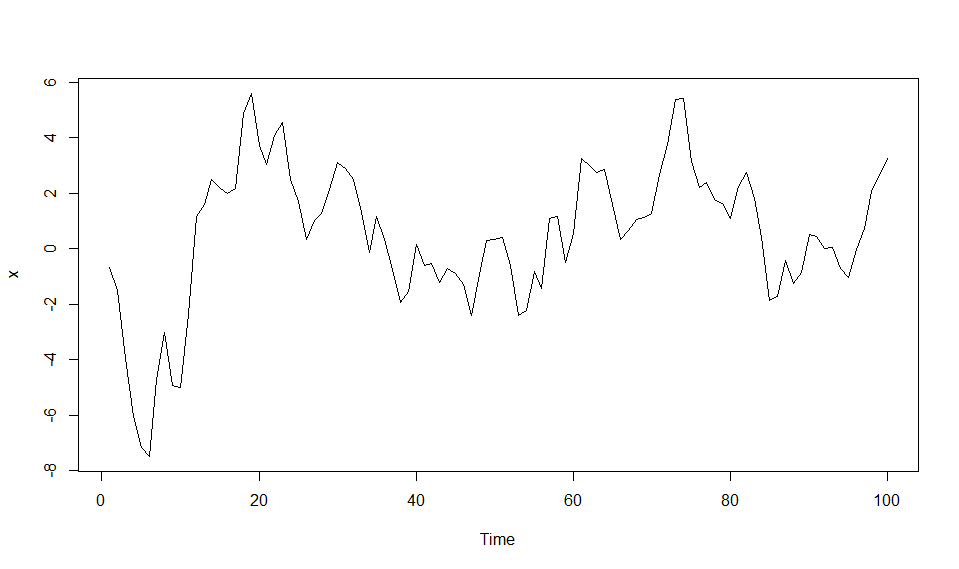
\includegraphics[width = 14cm ]{Figures/serie4.png} 
        \caption{Simulación del ARMA(1,1) con $\phi $= 0.8 y $\theta =$ 0.4}
        \label{Fig. 4.01}
    \end{figure} 
    Notemos que la simulación tiene un valle en valores de $t$ cercanos a 10, sin embargo no es problema porque parece que la simulación es homocedástica, por estacionaria, aunque buena parte de la serie se concentre por encima de 0.
    Además, se gráfica la función de autocorrelación muestral llamando \textit{acf(x)} junto con la función de autocorrelación teórica.
    \begin{lstlisting}
        acf(x)
        h <- 0:20
        lines(h, 0.88*(0.8)**(h-1), col="red")
    \end{lstlisting}
    Obtenemos 
    \begin{figure}[H] 
        \centering 
        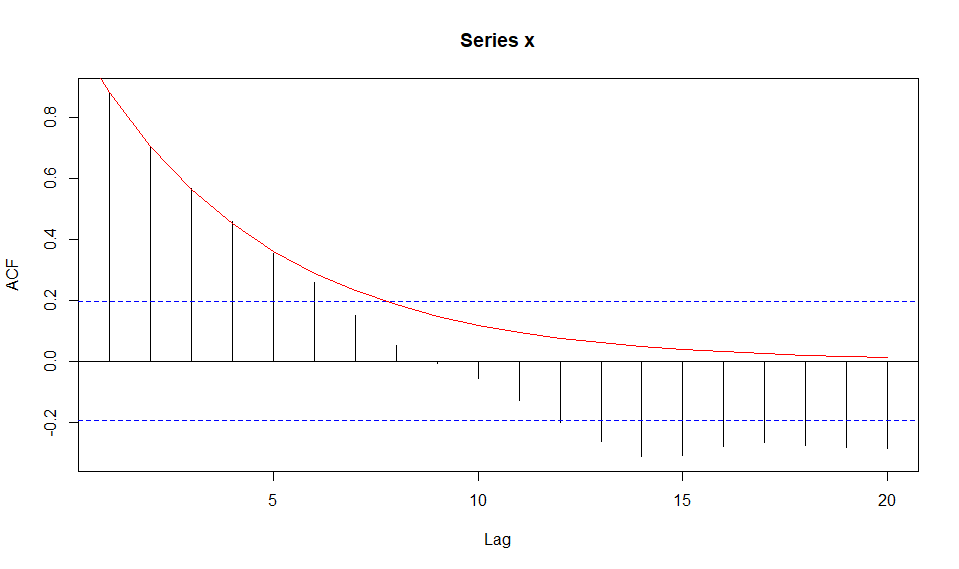
\includegraphics[width = 14cm]{Figures/acf4.png}     
        \caption{Función de autocorrelación muestral para la simulación del ARMA(1,1) y función de autocorrelación teórica.}
        \label{Fig. 4.02}
    \end{figure} 
    Se gráfica hasta el lag 20 y notemos que tenemos un cambio de signo para la autocorrelación para lag cercano a 15. Pero para valores de lag chicos el ajuste muestral contra el teórico es plausible.
    
    \item 
    Las ACF y PACF son útiles para identificar parámetros de procesos AR(p) y MA(q) puros. Sin embargo, para modelos mixtos se tiene una cantidad numerable de ceros, lo que hace difícil identificar los modelos de sus respectivas funciones muéstrales.

    El método de la función de autocorrelación extendida usa el hecho de que si se conoce la parte autoregresiva del modelo ARMA, entonces podemos filtrarlo en un modelo MA puro. Los coeficientes del AR se estiman por una secuencia finita de regresiones.

    Consideremos 
    \begin{align*}
        Y_t = \phi Y_{t-1} + e_t - \theta e_{t-1}
    \end{align*}
    En este caso, una simple regresión lineal de $Y_t$ en $Y_t-1$ resulta en una inconsistencia en el estimador de $\phi$. De hecho, de la ecuación (\ref{4.00}) sabemos que $\rho(1) = \left(\phi-\theta \right)(1-\phi \theta)/(1-2\phi \theta + \theta^2)$. El coeficiente de $Y_{t-1}$ en la segunda regresión, denotado por $\tilde{\phi}$ es un estimador consistente de $\phi$. Definamos $W_t = Y_t - \tilde{\phi}Y_{t-1}$, que es un modelo MA(1) aproximadamente. Para un ARMA(2,1), la tercera regresión de $Y_t$ en su primer lag con el residual del segundo lag de la primera regresión no da el coeficiente de $Y_{t-1}$ como estimador consistente de $\phi$. Similarmente, los coeficientes de un ARMA(p,q) pueden ser estimados consistentemente via una secuencia de $q$ regresiones.

    Como los ordenes del AR y MA son desconocidos, se requiere de un método iterativo. Sea
    \begin{align*}
        W_{t,k,j } = Y_t - \tilde{\phi}_1 Y_{t-1} - \cdots - \tilde{\phi}_k Y_{t-k }
    \end{align*}
    los residuales del modelo autorregresivo con los coeficientes estimados iterativamente suponiendo que AR es de orden $k$ y el orden del MA es $j$.  Para $k = p$ y $j\geq q$, $\{W_{t,j,k}\}$ es aproximadamente un modelo MA(q), entonces su autocorrelación teórica de lag $q+1$ o mayor son iguales a cero. Para $k>p$, ocurre una sobreparametrización del problema, y esto incrementa el orden del MA para el proceso $W$ por el mínimo de $k-p$ y $j-p$. Tsay y Tiao (1984) sugieren resumir la información de la función de autocorrelación extendida muestral en una tabla con el elemento en la $k$-ésima fila y $j$-ésima columna igual al símbolo $\times$ si el lag $j+1$ de la correlación muestral de $W_{t,k,j }$ es significativamente diferente de 0 (es decir, con magnitud mayor que 1.96/$\sqrt{n-j-k }$), en caso contrario se anota un 0. En dicha tabla, un proceso ARMA(p,q) tendrá un patrón teórico de triangulo de ceros, con vértice en la parte superior izquierda que corresponde a los ordenes del ARMA. \cite{Cryer}
    
    
    Para el caso particular de la simulación, obtenemos que la tabla generada por la EACF es
    \begin{figure}[H] 
        \centering 
        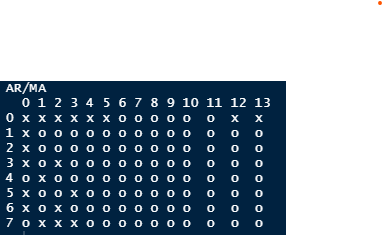
\includegraphics[width = 10 cm]{Figures/EACF.png} 
        \caption{Tabla de la función de autocorrelación extendida.}
        \label{Fig. 4.03}
    \end{figure} 
    Aunque es difícil detectar el patron triangular, intrínsecamente sabemos que debería ser una triangulo con punta en 1,1 por la simulación. Vemos que se puede ver una separación diagonal, sin embargo hay muchos ceros debajo de ella. Por tanto, me parece que la estimación en este caso según el EACF es (1,1)

    \item 
    Con una nueva semilla, volvemos a simular a 100 pasos para el mismo ARMA(1,1). Esta vez se obtiene la gráfica de la función de autocorrelación siguiente
    \begin{figure}[H] 
        \centering 
        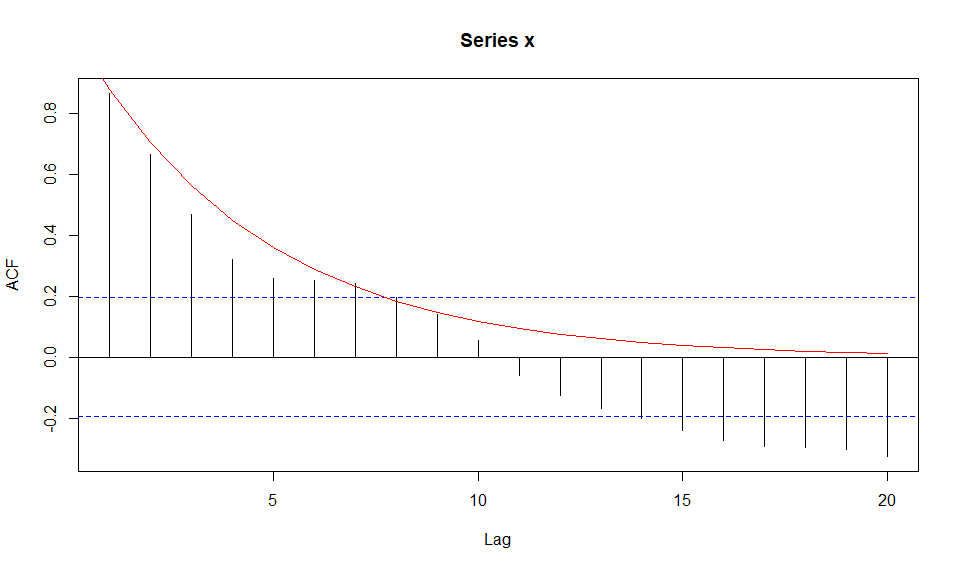
\includegraphics[width = 14 cm ]{Figures/ACF4_2.png}       
        \caption{Función de autocorrelación muestral y teórica para otra simulación del ARMA(1,1).} 
        \label{Fig. 4.04}
    \end{figure} 
    La tabla generado por el EACF es
    \begin{figure}[H] 
        \centering 
        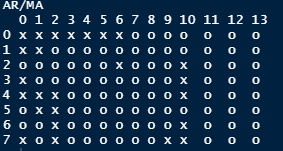
\includegraphics[width = 10 cm ]{Figures/EACF_2.png} 
        \caption{Tabla de la función de autocorrelación extendida.}
        \label{Fig. 4.05}
    \end{figure} 
    En este caso, no es claro la división triangular observamos que definitivamente por la parte superior el p se estima en 1 sin embargo para $q$ no es claro si se toma 0 o 1.

    \item 
    Para la simulación con $n = 48$ se obtiene la siguiente función de autocorrelación
    \begin{figure}[H] 
        \centering 
        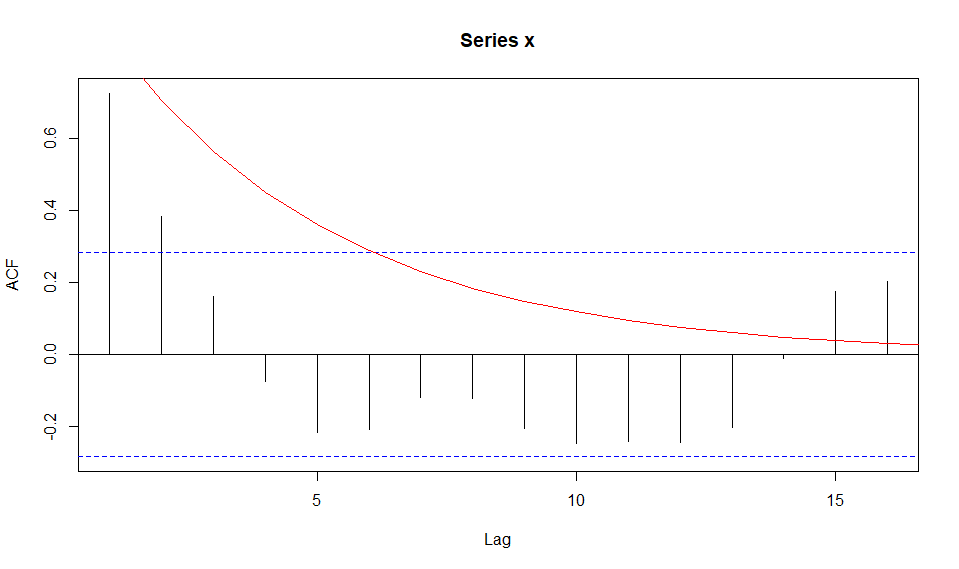
\includegraphics[width = 14 cm ]{Figures/acf_d.png} 
        \caption{Función de autocorrelación muestral y teórica para otra simulación del ARMA(1,1).}
        \label{Fig. 4.06}
    \end{figure} 
    Notamos un ajuste bastante pobre de la AFC muestral respecto al teórico.

    Ahora, para el EACF
    \begin{figure}[H] 
        \centering 
        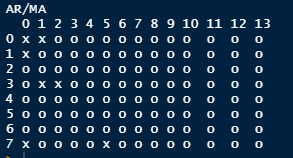
\includegraphics[width = 10 cm]{Figures/EAFC_d.png} 
        \caption{Tabla de la función de autocorrelación extendida.}
        \label{Fig. 4.07}
    \end{figure}  
    notamos que, aunque hay bastantes ceros, se alcanza a distinguir el pico en el (1,1) que es la estimación correcta.

    Para $n=200$ con la misma semilla, la función de autocorrelación es
    \begin{figure}[H] 
        \centering 
        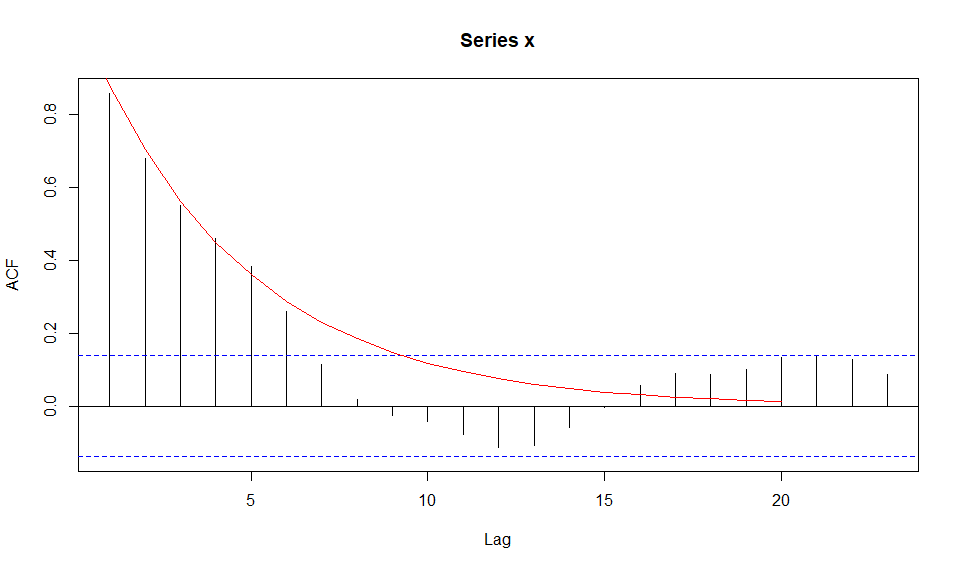
\includegraphics[width = 14 cm ]{Figures/ACF_d2.png} 
        \caption{Función de autocorrelación muestral y teórica para otra simulación del ARMA(1,1).}
        \label{Fig. 4.08}
    \end{figure} 
    que se observa un mejor ajuste entre el muestral y el teórico. Luego, el la tabla asociada a el EACF es
    \begin{figure}[H] 
        \centering 
        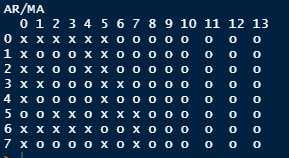
\includegraphics[width = 10 cm ]{Figures/EACF_D2.png} 
        \caption{Tabla de la función de autocorrelación extendida.}
        \label{Fig. 4.09}
    \end{figure} 
    Nuevamente, notamos que la fila superior esta bien definida, la diagonal se alcanza a distinguir, luego el estimador queda nuevamente en el (1,1) que es la estimación correcta.



\end{enumerate}

\end{solution}


\begin{problem}{6} 
    Sea $\{X_t : t = 0,\pm 1, \pm 2, \cdots \}$ definida como
    \begin{align*}
        X_t + \alpha X_{t-1} + \alpha_2 X_{t-2} = e_t \:\:\:\:\: e_t \sim \text{no-correlacionados}(0,\sigma^2).
    \end{align*}
    Sean $r_1, r_2$ las raíces (reales) con $|r_i|<1$, $i=1,2$. Muestra que 
    \begin{align*}
        X_t - r_1 X_{t-1} = Y_t 
    \end{align*}
    es un AR(1) con parámetro $r_2$.
\end{problem}

Reescribamos la serie de tiempo de la siguiente manera
\begin{align*}
    e_t &= X_t + \alpha_1 X_{t-1} + \alpha_2 X_{t-2} \\
    &= \left(1 + \alpha_1 B + \alpha_2 B^2  \right) X_t
\end{align*}
donde $B$ es el operador \textit{backshift}. Tenemos el polinomio característico $\phi (z) = 1+ \alpha_1 z+ \alpha_2 z^2$ con raíces reales $r_1,r_2$. Entonces, de algebra elemental podemos escribir el polinomio característico como 
\begin{align*}
    \phi(z) &= 1 - (r_1+r_2)z + r_1 r_2 z^2\\
    &= (1- r_1z)(1-r_2 z)
\end{align*}

Como $|r_1|<1$ y $|r_2| < 1$ por hipótesis, entonces
\begin{align*}
   0= 1 - r_1 z_1  \:\:\:\Leftrightarrow \:\:\: z_1 = \frac{1}{r_1}\:\:\: \Leftrightarrow \:\:\: |z_1| > 1 \\ 
   0= 1 - r_2 z_2  \:\:\:\Leftrightarrow \:\:\: z_2 = \frac{1}{r_2}\:\:\: \Leftrightarrow \:\:\: |z_2| > 1
\end{align*}

Recordemos en \cite{Chan} el siguiente:

\textbf{Teorema 3.2}

Un proceso AR($p$) es causal si las raíces del polinomio característico $\phi(z) = 1- \phi_1 z -\cdots - \phi_p z ^p$ todas están fuera del circulo unitario.

Por tanto, $X_t$ es un proceso causal. Recordemos además, que un proceso se dice causal si existen $\psi_j$ con $\sum_{j=0}^{\infty} |\psi_j | < \infty$ tal que 
\begin{align*}
    Y _t = \sum_{j=0}^{\infty} \psi_j e_{t-j} 
\end{align*}

Particularmente, hemos visto que la expansión para $Y_t = \phi Y_{t-1} + e_t $ un AR(1) causal de parámetro $\phi$ ($|\phi| < 1)$ tiene como expansión
\begin{align}
    Y_t = \sum_{j=0}^{\infty} \phi^j e_{t-j}
    \label{6.01}
\end{align}
es decir, $\psi_j = \phi^j$, pag. 30 \cite{Chan}.

Luego, volviendo a la serie de tiempo de interés. 
\begin{align*}
    X_t = \phi(B)^{-1}e_t = \frac{1}{(1-r_1 B)(1-r_2 B )}e_t .
\end{align*}
Por fracciones parciales 
\begin{align*}
    \frac{1}{(1-r_1z )(1-r_2 z )} &= \frac{A}{1-r_1z} + \frac{B}{1-r_2 z },\\
    &= \frac{A(1-r_2 z )+ B(1-r_1 z)}{(1-r_1 z)(1-r_2 z )}
\end{align*}
se sigue 
\begin{align*}
    1 = A(1-r_2 z )+ B(1-r_1 z)
\end{align*}
Resolviendo como es usual, propongamos $z = 1/r_2$ entonces
\begin{align*}
    1 = B \left(1- \frac{r_1}{r_2}\right)  \:\:\: \Leftrightarrow \:\:\: B = \frac{r_2}{r_2- r_1}
\end{align*}
proponiendo $z = 1/r_1$
\begin{align*}
    1 = A \left(1-\frac{r_2}{r_1}\right) \:\:\: \Leftrightarrow \:\:\: A = -\frac{r_1}{r_2-r_1}
\end{align*}
entonces
\begin{align*}
    \frac{1}{(1-r_1z )(1-r_2 z )} = \frac{1}{r_2-r_1}\left(\frac{r_2}{1-r_2 z } - \frac{r_1}{1- r_1 z}\right)
\end{align*}
La serie de tiempo queda entonces, expresada como
\begin{align}
    X_t &= \frac{1}{(1-r_1B )(1-r_2 B )} e_t \nonumber\\
    &= \frac{1}{r_2-r_1}\left(\frac{r_2}{1-r_2 B } - \frac{r_1}{1- r_1 B}\right) e_t\nonumber\\
    &= \frac{1}{r_2-r_1} \left( r_2 \sum_{j=0}^{\infty} r_2^j B^j- r_1\sum_{j=0}^{\infty}r_1^jB^j \right) e_t\nonumber\\
    &= \frac{1}{r_2-r_1} \sum_{j = 0}^{\infty} (r_2^{j+1}-r_1^{j+1}) e_{t-j }
    \label{6.02}
\end{align}
donde podemos notar que $\psi_j = (r_2^{j+1}-r_1^{j+1})/(r_2-r_1)$ para la expansión dada por la definición de causalidad.

Ahora, analizamos el siguiente proceso
\begin{align*}
    Y_t = X_t - r_1 X_{t-1}
\end{align*}
de la expansión en (\ref{6.02})
\begin{align*}
    Y_t &= \frac{1}{r_2-r_1} \sum_{j = 0}^{\infty} (r_2^{j+1}-r_1^{j+1}) e_{t-j } - r_1 \frac{1}{r_2-r_1} \sum_{j = 0}^{\infty} (r_2^{j+1}-r_1^{j+1}) e_{t-1-j }\\
    &= \frac{1}{r_2-r_1} \left( \sum_{j = 0}^{\infty} (r_2^{j+1}-r_1^{j+1}) e_{t-j } - \sum_{j =0 }^{\infty} (r_1r_2^{j+1}- r_1^{j+2} ) e_{t-(j+1)}\right) \\
    &= \frac{1}{r_2-r_1} \left( \sum_{j = 0}^{\infty} (r_2^{j+1}-r_1^{j+1}) e_{t-j } - \sum_{j =1 }^{\infty} (r_1r_2^{j}- r_1^{j+1} ) e_{t-j}\right)    
\end{align*}
donde se cambio la indentación a la segunda suma. Abriendo a el primer término para la primer suma y cancelando con la segunda
\begin{align*}
    Y_t &= \frac{1}{r_2-r_1} \left( (r_2 -r_1)e_t + \sum_{j = 1}^{\infty} (r_2^{j+1}-r_1^{j+1}) e_{t-j } - \sum_{j =1 }^{\infty} (r_1r_2^{j}- r_1^{j+1} ) e_{t-j}\right)\\
    &= \frac{1}{r_2-r_1} \left( (r_2 -r_1)e_t + \sum_{j = 1}^{\infty} r_2^{j+1} e_{t-j } - \sum_{j =1 }^{\infty} r_1r_2^{j}  e_{t-j}\right)\\
    &= \frac{1}{r_2-r_1} \left( (r_2 -r_1)e_t + \sum_{j = 1}^{\infty} (r_2-r_1)r_2^{j} e_{t-j } \right)\\
    &= e_t + \sum_{j=1}^{\infty} r_2^j e_{t-j}\\
    &= \sum_{j=0}^{\infty} r_2^j e_{t-j }
\end{align*}
Por tanto, tenemos la expansión de un proceso causal. De la relación (\ref{6.01}) podemos notar que $Y_t$ es un AR(1) de parámetro $\phi = r_2$ y 
\begin{align*}
    Y_t = r_2 Y_{t-1} + e_t 
\end{align*}
lo que concluye la demostración.


\begin{problem}{7} 
    Define el proceso $\{ X_t\}$ como $X_t = \sum_{j=0}^{\infty}\rho^j e_{t-j }(=\rho X_{t-1} + e_t )$, donde $e_t\sim$ no-correlacionadas $(0,\sigma^2_e)$ y $ |\rho |<1 $. Sea $u_t$ una sucesión de v.a. no-correlacionadas $(0,\sigma^2_u)$ independientes de $\{e_t\}$. Sea $Y_t = X_t + u_t$ (i.e. $Y_t$ es $X_t$ medida con un error $u_t$). 
    \begin{enumerate}
        \item Encuentra la función de autocovarianza de $Y_t$. 
        \item Encuentra un proceso ARMA(1,1) $Z_t = \alpha_1 Z_{t-1} + \beta_1 e_{t-1} + e_t $, donde $e_t \sim$ no-correlacionadas($0,\sigma^2_\epsilon$) tal que $\gamma_Z(h ) = \gamma_Y(h )$ para toda $h$.
        \item Si $X_t$ fuera un ARMA(p,q) estacionario e invertible, ?`qué puedes decir de $Y_t = X_t + u_t $? donde $u_t$ es WN$(0,\sigma^2_u )$ independiente de $X_t$. 
    \end{enumerate} 
\end{problem}

\begin{solution} 
    \begin{enumerate}
        \item 
        Como $X_t$ es un AR(1) causal ya hemos calculado su función de covarianza, esta es
        \begin{align*}
            \gamma_X(h )= \sigma_e^2 \frac{\rho^h }{1-\rho^2}
        \end{align*}
        Luego, calculando la función de covarianza para $Y_t$
        \begin{align*}
            \gamma_Y(h ) &= Cov(Y_{t},Y_{t+h }) ,\\
            &= Cov(X_t + u_t, X_{t+h }+ u_{t+h }),\\
            &= Cov(X_t, X_{t+h }) + Cov(X_t, u_{t+h }) + Cov(u_t, X_{t+h }) + Cov(u_t, u_{t+h })
        \end{align*}
        como $X_t$ es independiente de $u_t$
        \begin{align}
            \gamma_Y(h ) &= \gamma_X (h ) + Cov(u_t,u_{t+h }), \nonumber\\
            &= \sigma_e^2 \frac{\rho ^h }{1-\rho^2} + \sigma_u^2 \delta(h).
            \label{7.01}
        \end{align}
        \item 
        Para este caso, de pag. 72 en \cite{Fuller} tenemos que la función de autocovarianza para el ARMA(1,1) invertible y causal
        \begin{align*}
            Z_t = -\alpha Z_{t-1} + \varepsilon_t +\beta \varepsilon_{t-1}
        \end{align*}
        es
        \begin{align}
            \gamma_Z(h ) = 
            \left\{\begin{matrix}
                \frac{1+ \beta^2 + 2\beta\alpha}{1-\alpha^2} \sigma_\varepsilon^2, & h = 0 \\ 
                \frac{(1+\beta\alpha)(\alpha + \beta)}{1-\alpha^2} \alpha^{h-1}\sigma^2_{\varepsilon } ,& h = 1,2,\cdots 
            \end{matrix}\right.
            \label{7.02}
        \end{align}
        por lo que el proceso será tal que resuelva el sistema de ecuaciones comparando (\ref{7.01}) y (\ref{7.02}).

        \item 
        Como $X_t$ es un ARMA(p,q) entonces existen polinomios $\phi(B), \theta(B)$ de orden $p,q$, respectivamente con raíces fuera del circulo unitario tal que
        \begin{align*}
            \phi(B) X_t = \theta(B) e_t.
        \end{align*} 
        Entonces
        \begin{align*}
            \phi(B)Y_t &= \phi(B)(X_t + u_t),\\
            &= \phi(B)X_t + \phi(B)u_t,\\
            &= \theta(B)e_t + \phi(B )u_t,
        \end{align*}
        por tanto, del lado izquierdo mantenemos un AR(p) mientras que en el lado derecho tenemos un MA(r) donde $r= \max\{p,q\}$ ya que tenemos la suma de dos MA independientes.


    \end{enumerate}
\end{solution}
    


\begin{problem}{8} 
    El conjunto de datos deere3 contiene 57 mediciones consecutivas registradas en una máquina de la compañía Deere and Co. Los valores están dados en desviaciones de un valor ideal en diezmillonésimas de una pulgada. El proceso emplea un mecanismo de control que reinicia algunos parámetros de la máquina dependiendo de la magnitud de la desviación del valor ideal del último ítem producido. Los datos están disponibles en el paquete TSA de R.
    \begin{enumerate}
        \item Grafica la ST y comenta al respecto. ?` Un modelo estacionario es apropiado?
        \item Grafica la ACF y PACF para esta serie y selecciona los órdenes tentativos de un modelo ARMA para la serie. 
        \item Selecciona el orden empleando un criterio distinto o alguno que complemente el inciso anterior.
    \end{enumerate}


\end{problem}

\begin{solution} 
La grafica de la serie de tiempo es  
\begin{figure}[H] 
    \centering 
    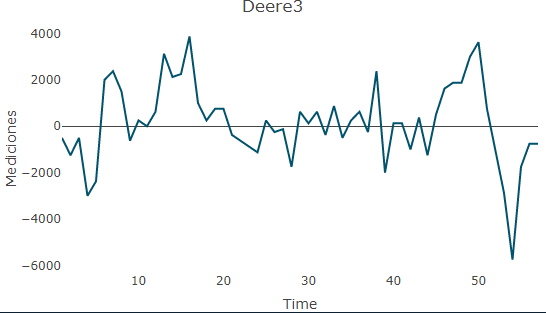
\includegraphics[width = 14cm]{Figures/Deere.png} 
    \caption{Serie temporal para las mediciones consecutivas de una máquina de Deere and co.}
    \label{Fig. 8.1}
\end{figure} 
podemos ver que parece tener una esperanza centrada en cero, por lo que pudiéramos pensar que es estacionaria. Sin embargo, notemos que parece ser un proceso heterocedástico debido a que la varianza por la medición 50 es mayor que en en el resto. Sin embargo, podemos pensar que dicha observación se debe a que el ruido blanco detrás puede ser un ruido de cola ligera y está es una observación atípica. Entonces, aún podemos dar el supuesto de estacionaridad y ajustar un modelo ARMA. Para ello veamos el ACF y PACF 

\begin{figure}[H] 
    \centering 
    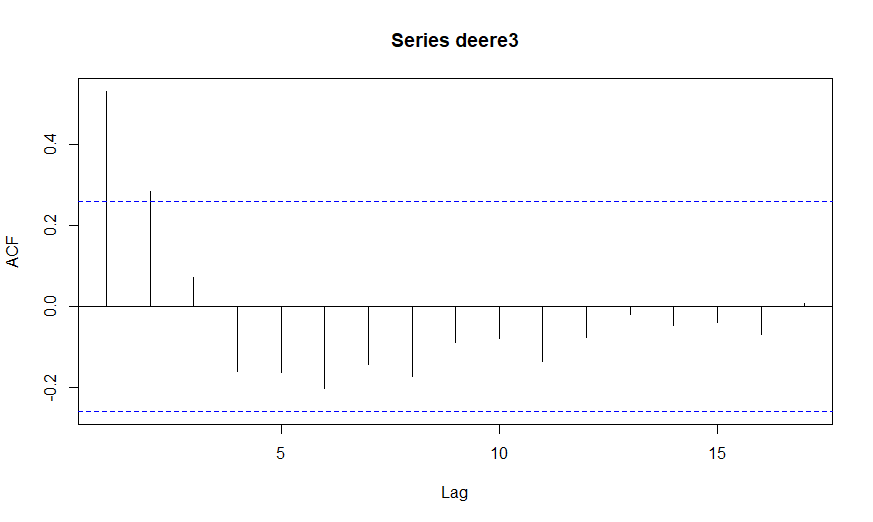
\includegraphics[width = 14cm ]{Figures/ACF8.png} 
    \caption{Función de autocorrelación para la los datos de Deere.}        
    \label{Fig. 8.2}
\end{figure} 

\begin{figure}[H] 
    \centering 
    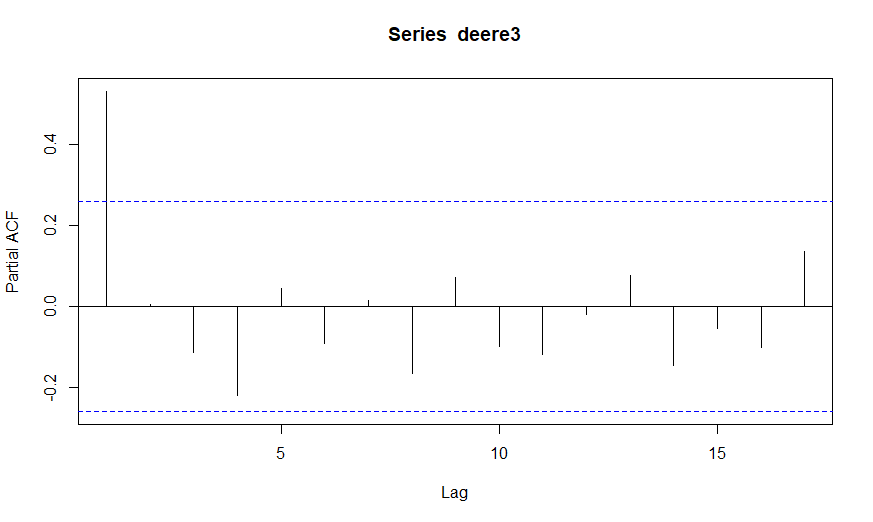
\includegraphics[width = 14cm]{Figures/PACF8.png} 
    \caption{Función de autocorrelación parcial para la serie de Deere.}
    \label{Fig. 8.3}
\end{figure} 
\end{solution}
    
Posteriormente, para calcular el orden de selección, usamos los ordenes que minimicen el AIC.
Con el siguiente ciclo, calculamos el AIC del modelo para las combinaciones posibles de modelos con p,q de cero a cuatro
\begin{lstlisting}
for (i in 0:4) for (j in 0:4) {
    current.aic <- AIC(arima(x, order=c(i, 0, j)))
    if (current.aic < final.aic) {
        final.aic <- current.aic
        final.order <- c(i, 0, j)
        final.arma <- arima(x, order=final.order)
}
}
\end{lstlisting}
lo que nos da que el mejor orden es $p = 3,  q =1$.
Finalmente, con la prueba de Ljung-Box testeamos que se tenga un buen ajuste. Con el comando 
\begin{lstlisting}
    Box.test(resid(final.arma), lag=20, type="Ljung-Box")
\end{lstlisting}
lo que nos da
\begin{lstlisting}

    Box-Ljung test

    data:  resid(final.arma)
    X-squared = 6.4666, df = 20, p-value = 0.9981
    
\end{lstlisting}
que tiene un p-valor mayor al nivel de significancia de 0.05. Por tanto, aceptamos los ordenes del modelo.

Por otro lado, para buscar ordenes de otra forma empleamos el EACF cuya tabla se muestra a continuación
\begin{figure}[H] 
    \centering 
    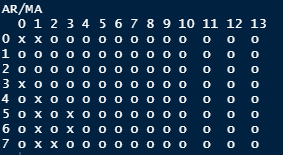
\includegraphics[width = 10 cm ]{Figures/EACF8.png} 
    \caption{Tabla para la estimación de ordenes por medio de la función de autocorrelación extendida.}
    \label{Fig. 8.1}
\end{figure} 
Notamos que el estimador no es categórico, ya que de puede ver una linea difusa, entonces podemos estimar que p = 2 ,q = 0.

\begin{thebibliography}{9}

    \bibitem{Chan}
    Chan, N. H. (2011). Time series: Applications to finance with R and S-Plus (Vol. 837). John Wiley and Sons.
  
    \bibitem{Brockwell}
    Brockwell, P. J., and Davis, R. A. (Eds.). (2002). Introduction to time series and forecasting. New York, NY: Springer New York.

    \bibitem{Fuller}
    Fuller, W. A. (2009). Introduction to statistical time series. John Wiley and Sons.

    \bibitem{Cryer}
    Chan, K. S., and Cryer, J. D. (2008). Time series analysis with applications in R. springer publication.
\end{thebibliography}

    


\end{document}